

In this section we demonstrate that the proof system presented in section \ref{sect:proofSystem} is sound. 
For this, we give a stronger meaning to our Hoare tuples  (Sect \ref{s:scoped:valid}), we require  that an  assertion hold from the perspective of \emph{several frames}, rather than just the top frame.

We prove soundness  of Hoare triples (Sect \ref{sect:prove:triples:sound}).
We then show how execution starting from some external state can be summarised into purely external execution and terminating execution of public methods (Sect \ref{sect:termExecs}). We then use these decompositions and a well-founded ordering to prove soundness of our quadruples  and of the overall system (Sect \ref{sect:prove:sound:quadruples}).


\subsection{\Strong Satisfaction} 
\label{s:scoped:valid}


As shown in section~\ref{s:viewAndProtect}, an assertion which held at the end of a method execution, need not hold upon return from it -- \cf Ex. \ref{ex:pop:does:not:preserve}.  

\begin{example}[$Stb^+$ not always preserved by Method Return]
\label{ex:motivate:scopes}
Assume state $\sigma_a$, such that $\interpret {\sigma_a} {\prg{this}}=o_1$, $\interpret {\sigma} {\prg{this}.f}=o_2$, $\interpret {\sigma} {x}=o_3$, $\interpret {\sigma} {x.f}=o_2$,  
and $\interpret {\sigma} {x.g}=o_4$, where $o_2$ is external and all other objects are internal. 
We then have $..,\sigma_a \models  \inside {o_4}$.
Assume %that
 the continuation of $\sigma_a$   consists of a method $x.m()$. Then,
upon entry to that method, when we push the new frame, we have  state $\sigma_b$, which also satisfies $..,\sigma_b \models  \inside {o_4}$.
Assume % that
 the   body of $m$ is $\prg{this}.f.m1(\prg{this}.g); \prg{this}.f := \prg{this};  \prg{this}.g := \prg{this}$, and % that 
 the external method $m1$ stores in the 
receiver a reference to the argument.
Then, at the end of method execution, and before popping the stack, we have   state $\sigma_c$, which also satisfies $..,\sigma_c \models  \inside {o_4}$.
However, after we pop the stack, we obtain $\sigma_d$, for which $..,\sigma_d \not\models  \inside {o_4}$.
\end{example} 


 

To address this problem, we introduce \emph{scoped satisfaction}: % of assertions: 
 $ \satDAssertFrom M  \sigma k   A$   says that $A$ is satisfied in $\sigma$  in all frames of $\sigma$ from $k$ onwards, 
\ie  $ \satDAssertFrom M  \sigma k   A$ iff $\sigma = ((\phi_1\cdot ... \phi_n), \chi)$ and $k\leq n$ and $\forall j. [\  k\leq j \leq n \ \Rightarrow \ M, ((\phi_1\cdot ... \phi_j), \chi) \models A'\ ]$ where $A'$ is $A$ whose free variables have been substituted according to $\phi_n$ -- \cf Def. \ref{def:restrict}.
We also introduce ``\strong'' quadruples,   $\satisfiesD {M} {\quadruple  {A} }   {\sigma}   {A'} {A''}$, which promise that if $\sigma$ satisfies $A$ from $k$ onwards, and executes its continuation to termination, then the final state will satisfy $A'$ from $k$ onwards, and also, all intermediate external states will satisfy $A''$ from $k$ onwards - \cf Def \ref{def:restrict}.
% We define   $\satisfiesD {M} {\quadruple  {A} }   {stmt}   {A'} {A''} $ and  $\satisfiesD {M} {S}$ accordingly.


Thus. continuing with example \ref{ex:motivate:scoped},  we have that\ \  $\satisfies {M} {\quadruple   {\inside {o_4}} }   {\sigma_b}   {\inside {o_4}}  {true} $, \ \ 
 but \\ $\notSatisfiesD {M}   {\quadruple   {\inside {o_4}} }  {\sigma_b}   {\inside {o_4}}  {true}  $.
\ \  In general, \strong satisfaction is stronger than shallow:   
 
\begin{lemma}[\strong   vs Shallow Satisfaction]
For all $M$, $A$, $A'$, $A''$, $\sigma$, $stmt$, and $S$
\begin{itemize}
\item
 $\satisfiesD {M} {\quadruple  {A} }   {\sigma}   {A'} {A''}   \ \ \ \Longrightarrow \ \ \   \satisfies {M} {\quadruple  {A} }   {\sigma}   {A'} {A''}$

%\item
% $\satisfiesD {M} {\quadruple  {A} }   {stmt}   {A'} {A''}   \ \ \ \Longrightarrow \ \ \   \satisfies {M} {\quadruple  {A} }   {stmt}   {A'} {A''}$
%\item 
%$\satisfiesD {M} {S}  \ \ \ \Longrightarrow \ \ \ \satisfies {M} {S}$
\end{itemize}
\end{lemma}

 %%%%%%%%

\subsection{Soundness of the Hoare Triples Logic}
\label{sect:prove:triples:sound}

We require a  proof system for assertions, $M\vdash A$, and expect it to be sound.
We also expect  the    underlying Hoare logic,  $M\ \vdash_{ul}\  \triple A {stmt} {A'}$,   to be be  sound, \cf Axiom \ref{ax:ul:sound}.
We then prove various properties about protection -- \cf section \ref{s:app:protect:lemmas} --  and finally prove 
 soundness of the inference system for triples $M \vdash  \triple A {stmt} {A'} $ -- \cf \A, \ref{s:sound:app:triples}.

 

\begin{Theorem}
\label{l:triples:sound}
For module  $M$   such that  $\vdash M$, and for any assertions $A$,  $A'$, $A''$ and statement  $stmt$:
\begin{center}
$M\ \vdash\  \triple A {stmt} {A'}  \ \ \ \  \Longrightarrow  \ \ \ \ \satisfiesD {M} {\quadruple {A} {stmt} {A'} {A''}}$
\end{center}
\end{Theorem}
 

\subsection{Summarised Execution}
\label{s:summaized}

When proving soundness of the external call rule, we are faced with the challenge that
execution of an external call may consist of any number of external
steps, interleaved with calls to public internal methods, which in
turn may make any number of further internal calls (whether public or private), and these, again may call external methods.
% Thus, execution of an external call will involve several internal and external states.
 


\label{sect:termExecs}


\vspace{.1cm}

\begin{tabular}{lll}
\begin{minipage}{.44\textwidth}
The diagram opposite shows such an execution:
  $ \leadstoBoundedStarFin {\Mtwo\cdot M}    {\sigma_2}  {\sigma_{30}}$ consists of 
 \textbf{three} public internal calls, and    {four} external calls,.%4 calls to external objects,
%and  . % 3 calls to internal objects.
%The external calls %to external objects 
%are from $\sigma_2$ to $\sigma_3$,  from $\sigma_3$ to $\sigma_4$, from $\sigma_9$ to $\sigma_{10}$, 
%and  from $\sigma_{16}$ to $\sigma_{17}$.
 The internal calls %to internal objects 
 are from $\sigma_5$ to $\sigma_6$, from $\sigma_7$ to $\sigma_8$, and from $\sigma_{21}$ to $\sigma_{23}$. 
\end{minipage}
& \ \  &
\begin{minipage}{.4\textwidth}
\resizebox{6.3cm}{!}
{
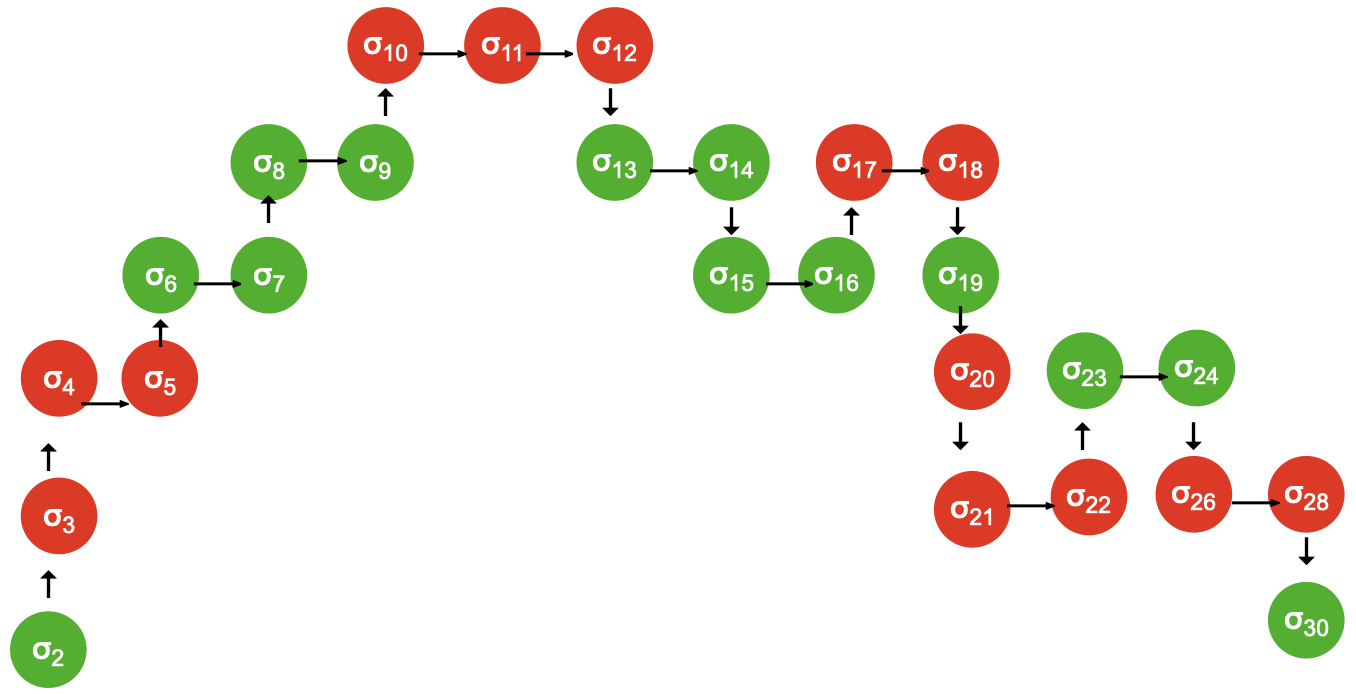
\includegraphics[width=\linewidth]{diagrams/summaryA.png}
} \end{minipage}
\end{tabular}
 
\vspace{.1cm}


 
When proving soundness of   rule {\sc{Call\_Ext}}, % and  {\sc{Call\_Ext\_Adapt}}
we   use that  $M \vdash \encaps A$ (and also \strong satisfaction)  to argue that 
external transitions (from one external state to another external state)  preserve $A$. 
For calls from external states to internal methods (as in $\sigma_5$ to $\sigma_6$), 
we want to apply the fact that the method body has been proven to preserve $A$ (by  {\sc{Method}}).
That is, for the external states we consider small steps, while for each of the public method calls we want to consider large steps --
in other words, we notionally \emph{summarize} the calls of the public methods into one large step.
  Moreover, for the external states we apply different arguments than for the internal states.

%\vspace{.1cm}
% In this subsection we define some auxialliary concepts to express summarized execution, and prove  associated  lemmas.
  
\begin{tabular}{lll}
\begin{minipage}{.44\textwidth}
 In terms of our example, we  summarise the execution into \textbf{two} public internal calls.
  % through of the
 % two ``outer'' internal, public methods into the 
 the ``large'' steps $\sigma_6$ to $\sigma_{19}$ and $\sigma_{23}$ to $\sigma_{24}$.
 % And are not concerned with the states reached from these two public method executions.  
\end{minipage}
& \ \  &
\begin{minipage}{.4\textwidth}
\resizebox{6.3cm}{!}
{
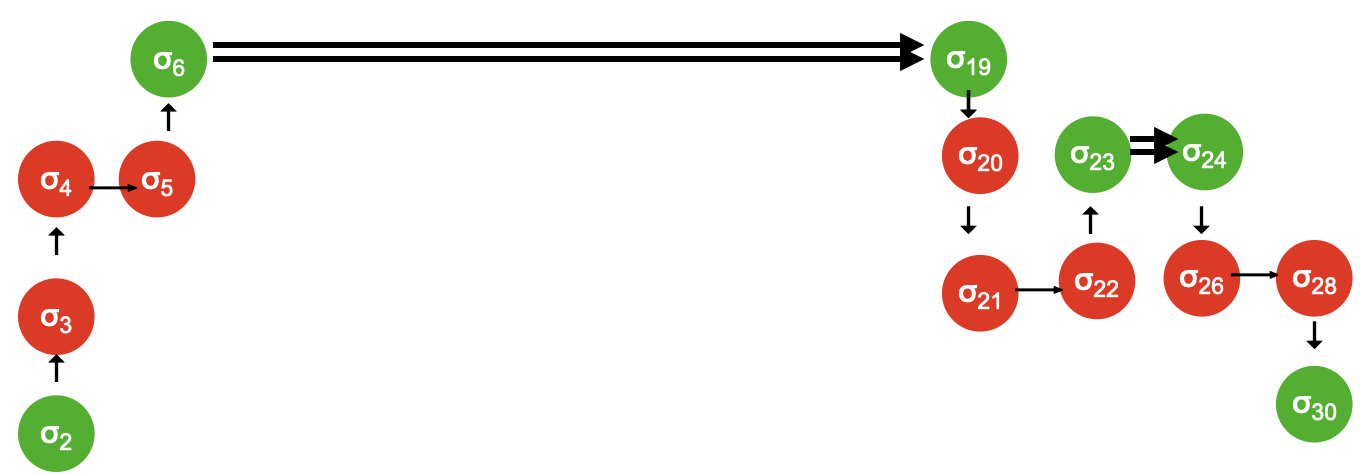
\includegraphics[width=\linewidth]{diagrams/summaryB.png}
} \end{minipage}
\end{tabular} 

 \vspace{.15cm}

\noindent 
In order to express such summaries, Def. \ref{def:exec:sum} introduces \emph{summarized} executions, whereby\\ 
%\begin{itemize}
%\item
$\strut \ \ \  \WithExtPub {\Mtwo\cdot M} {\sigma\bd}  {\sigma}  {\sigma'} {\sigma_1...\sigma_n}$  \ \  \  \ says that $\sigma$ reaches $\sigma'$ through 
external states, interleaved with summarised public internal method calls, starting at ${\sigma_1...\sigma_n}$, respectively.
% end{itemize}
% \noindent
%
In our example, we have 
 $\strut \ \ \  \WithExtPub {\Mtwo\cdot M} {\sigma_2}  {\sigma_{2}}   {\sigma_{20}}  {\sigma_5,\sigma_{21}}$.


\vspace{.1cm}

% We now revisit external executions interleaved with public method calls:   
%In the appendix, we prove 
Lemma \ref{lemma:external_breakdown:term} from  the  Appendix   says that any terminating execution
% ,  $ \leadstoBoundedStarFin {\Mtwo}  {\sigma}  {\sigma'}$, 
 starting in an external state  consists of a  sequence of  external states interleaved with terminating executions
 %  in internal states, 
% $\WithExtPub {\Mtwo\cdot M} {\sigma\bd}  {\sigma}  {\sigma'} {\sigma_1...\sigma_n}$.
of public methods.
Lemma  \ref{lemma:external_exec_preserves_more} says that an encapsulated assertion $A$  is preserved by an execution
% $\WithExtPub {\Mtwo\cdot M} {\sigma\bd}  {\sigma}  {\sigma'} {\sigma_1...\sigma_n}$, 
starting at an external state provided that all finalising internal executions  %(the public methods called at $\sigma_1$, ... $\sigma_n$) 
also preserve $A$: that is, if $A$ is encapsulated, 
 and $\WithExtPub {\Mtwo\cdot M} {\sigma\bd}  {\sigma}  {\sigma'} {\sigma_1...\sigma_n}$, and 
 the calls at  $\sigma_1$, ... $\sigma_n$ preserve $A$,  then $A$ is preserved from $\sigma$ to $\sigma'$.  
% It is used to prove  soundness of the rule {\sc{ExtCall}}\footnoteSD{perhaps also {\sc{ExtCall\_WithSpec\_Strong}}}
% 
%In the appendix we prove lemmas \ref{lemma:external_breakdown:term} and \ref{lemma:external_exec_preserves_more} 
%which guarantee  that if $\sigma$ is external and $ \leadstoBoundedStarFin {\Mtwo}  {\sigma}  {\sigma'}$, 
%then there exist $\sigma_1$, ... $\sigma_n$, such that
% $\WithExtPub {\Mtwo\cdot M} {\sigma\bd}  {\sigma}  {\sigma'} {\sigma_1...\sigma_n}$.
% Conversely, if $A$ is encapsulated, 
% and $\WithExtPub {\Mtwo\cdot M} {\sigma\bd}  {\sigma}  {\sigma'} {\sigma_1...\sigma_n}$, and 
% the calls at  $\sigma_1$, ... $\sigma_n$ preserve $A$,  then $A$ is preserved from $\sigma$ to $\sigma'$.
  


  %%%%%%%%%%%%%%%%%%%%%%%%%%%%%%%%%%%%%%%%%%%%%%%%%%%

\subsection{ Soundness of the Hoare Quadruples Logic}

Another challenge when proving soundness of our quadruples is that the proof of some cases  requires induction on the execution while the proof of other cases  requires induction on the quadruples
proof.  We address this challenge  through  a well-founded ordering that combines both.
\label{sect:prove:wellfounded}
\label{sect:prove:sound:quadruples}
In Def.  \ref{def:measure}  we define that $(A_1,\sigma_1,A_2, A_3) \ll_{M,\Mtwo}  (A_4,\sigma_2,A_5, A_6)$ if $\sigma_1$ executes to termination  in fewer steps than $\sigma_2$ (considering the shortest scoped executions), or  the proof of $M \vdash \quadruple {A_1} {\sigma.\prg{cont}} {A_2} {A_3} $
is shallower than that of  $M \vdash \quadruple {A_4} {\sigma.\prg{cont}} {A_5} {A_6} $ (considering the shallowest proofs).  
The relation $\_ \ll_{M,\Mtwo}  \_$  is well-founded -- \cf lemma \ref{lemma:normal:two}
 

\begin{theorem}
\label{t:quadruple:sound}
\label{thm:soundness}
For module  $M$,   assertions $A$, $A'$, $A''$,   state  $\sigma$, and specification $S$:

\begin{enumerate}[(A)]
\item
 $:\strut \   \vdash M  \ \ \ \wedge \ \ \  M\ \vdash\  \quadruple {A} {stmt} {A'} {A''}  \ \ \ \ \ \ \ \Longrightarrow \ \ \ \ \ \  \ \ \  M\ \modelsD\  \quadruple {A} {stmt} {A'} {A''}$
 \item
  $:\strut \  \  \proves{M}{S}\ \ \ \ \ \ \Longrightarrow\ \ \ \ \ \  \ \ \ {M} \modelsD {S}$
 
\end{enumerate}

\end{theorem}

The proofs make use of summarized executions, well-founded orderings, and various assertion preservation properties. They can be found in App. \ref{s:app:proof:sketch;quadruples}
  %%%%%%%%%%%%%%%%%%%%%%%%%%%%%%%%%%%%%%%%%%%%%%%%%%%
%%  \subsection{Soundness of the overall system}
%\label{sect:prove:triples:overall}
%\noindent
%Finally, we  prove soundness of the overall system:
%
%\begin{theorem}[Soundness]
%\label{thm:soundness}
%%Assume an \SpecO proof system, $\proves{M}{A}$, 
%%an encapsulation inference system, $\proves{M}{\encaps{A}}$,
%%% Axiom xx, and 
%% and  that on top of these systems we built
%% the \SpecLang logic according to zzzz,  then, for    all modules $M$, and all \SpecLang specifications  $S$:
% For any module $M$, and specification $S$:
% 
% $$\proves{M}{S}\ \ \ \ \ \ \ \mbox{implies}\ \ \ \ \ \  \ \ \ {M} \modelsD {S}$$
%\end{theorem}
%
%We now prove soundness of the inference system $M \vdash  \quadruple A {stmt} {A'} {A''}$, using summarized executions from the earlier section, and the ordering $_ \ll \_$:   Proof outlines for these theorems can be found in \A \ref{s:app:proof:sketch;quadruples} and \ref{s:app:proof:sketch;overall}. 

%
%Theorem. \ref{thm:soundness} demonstrates 
% that the   \SpecLang logic is sound with respect to the semantics of \SpecLang specifications.
% The \SpecLang logic parametric wrt to the algorithms for proving validity of assertions
% $\proves{M}{A}$, and 
% assertion encapsulation ($\proves{M}{\encaps{A}}$), and is sound
% provided that these two proof systems are sound.
